%%========================================================================
%% LaTeX sjabloon voor stage/projectrapport of bachelorproef
%%  HoGent Bedrijf en Organisatie
%%========================================================================

%%========================================================================
%% Preamble
%%========================================================================

\documentclass[pdftex,a4paper,12pt,twoside]{report}

% XXX: Let op: dit sjabloon is gemaakt om dubbelzijdig af te drukken
% Voor enkelzijdig, verwijder ``twoside'' hierboven.

%%---------- Extra functionaliteit ---------------------------------------

\usepackage[utf8]{inputenc}  % Accenten gebruiken in tekst (vb. é ipv \'e)
\usepackage{amsfonts}        % AMS math packages: extra wiskundige
\usepackage{amsmath}         %   symbolen (o.a. getallen-
\usepackage{amssymb}         %   verzamelingen N, R, Z, Q, etc.)
\usepackage[dutch]{babel}    % Taalinstellingen: woordsplitsingen,
                             %  commando's voor speciale karakters
                             %  ("dutch" voor NL)
\usepackage{eurosym}         % Euro-symbool €
\usepackage{geometry}
\usepackage{graphicx}        % Invoegen van tekeningen
\usepackage{wrapfig}         % Positioneren van tekeningen
\usepackage[pdftex,bookmarks=true]{hyperref}
                             % PDF krijgt klikbare links & verwijzingen,
                             %  inhoudstafel
\usepackage{listings}        % Broncode mooi opmaken
\usepackage{multirow}        % Tekst over verschillende cellen in tabellen
\usepackage{rotating}        % Tabellen en figuren roteren
\usepackage{natbib}          % Betere bibliografiestijlen
\usepackage{fancyhdr}        % Pagina-opmaak met hoofd- en voettekst

\usepackage[T1]{fontenc}     % Ivm lettertypes
\usepackage{lmodern}
\usepackage{textcomp}

\usepackage{lipsum}          % Voor vultekst (lorem ipsum)

%%---------- Layout ------------------------------------------------------

% hoofdingen, enz.
\pagestyle{fancy}
% enkel hoofdstuktitel in hoofding, geen sectietitel (vermijd overlap)
\renewcommand{\sectionmark}[1]{}

% lijn, wordt gebruikt in titelpagina
\newcommand{\HRule}{\rule{\linewidth}{0.5mm}}

% Leeg blad
\newcommand{\emptypage}{
\newpage
\thispagestyle{empty}
\mbox{}
\newpage
}

% Gebruik een schreefloos lettertype ipv het "oubollig" uitziende
% Computer Modern
\renewcommand{\familydefault}{\sfdefault}

%%---------- Documenteigenschappen ---------------------------------------
%% Vul dit aan met je eigen info:

% Je eigen naam
\newcommand{\student}{Michiel De Wilde}

% De naam van je lector, begeleider, promotor
\newcommand{\promotor}{Bert Van Vreckem}

% De naam van je co-promotor
\newcommand{\copromotor}{Micha Hernandez van Leuffen}

% Indien je bachelorproef in opdracht van een bedrijf of organisatie
% geschreven is, geef je hier de naam.
\newcommand{\instelling}{Hogeschool Gent}

% De titel van het rapport/bachelorproef
\newcommand{\titel}{Unikernels}

% Datum van indienen
\newcommand{\datum}{29 mei 2015}

% Faculteit
\newcommand{\faculteit}{Faculteit Bedrijf en Organisatie}

% Soort rapport
\newcommand{\rapporttype}{Scriptie voorgedragen tot het bekomen van de graad van\\Bachelor in de toegepaste informatica}

% Academiejaar
\newcommand{\academiejaar}{2015-2016}

% Examenperiode
%  - 1e semester = 1e examenperiode
%  - 2e semester = 2e examenperiode
%  - tweede zit = 3e examenperiode
\newcommand{\examenperiode}{2e examenperiode}

%%========================================================================
%% Inhoud document
%%========================================================================

\begin{document}

%%---------- Front matter ------------------------------------------------
%% Het voorblad - Hier moet je in principe niets wijzigen.

\begin{titlepage}
  \newgeometry{top=2cm,bottom=1.5cm,left=1.5cm,right=1.5cm}
  \begin{center}

    \begingroup
    \rmfamily
    
\includegraphics[width=2.5cm]{img/HG-beeldmerk-woordmerk}\\[.5cm]
    \faculteit\\[3cm]
    \titel
    \vfill
    \student\\[3.5cm]
    \rapporttype\\[2cm]
    Promotor:\\
    \promotor\\
    Co-promotor:\\
    \copromotor\\[2.5cm]
    Instelling: \instelling\\[.5cm]
    Academiejaar: \academiejaar\\[.5cm]
    \examenperiode
    \endgroup

  \end{center}
  \restoregeometry
\end{titlepage}

% Schutblad

\emptypage


\begin{titlepage}
  \newgeometry{top=5.35cm,bottom=1.5cm,left=1.5cm,right=1.5cm}
  \begin{center}

    \begingroup
    \rmfamily
    \faculteit\\[3cm]
    \titel
    \vfill
    \student\\[3.5cm]
    \rapporttype\\[2cm]
    Promotor:\\
    \promotor\\
    Co-promotor:\\
    \copromotor\\[2.5cm]
    Instelling: \instelling\\[.5cm]
    Academiejaar: \academiejaar\\[.5cm]
    \examenperiode
    \endgroup

  \end{center}
  \restoregeometry
\end{titlepage}


\begin{abstract}
% TODO: De "abstract" of samenvatting is een kernachtige (max 1 blz. voor een
% thesis) synthese van het document. In ons geval beschrijf je kort de
% probleemstelling en de context, de onderzoeksvragen, de aanpak en de
% resultaten.
\end{abstract}

\chapter*{Voorwoord}
\label{ch:voorwoord}

Deze bachelorproef is tot stand gekomen uit eigen interesse. Computers hebben mij in mijn jeugd altijd al gefascineerd. Het heeft een tijd geduurd vooraleer ik begon met programmeren. Ik begon met de simpele applicatie maar al snel werd het meer complex.  Het beheren van servers en infrastructuur was een uitdaging die ik zeker aanging. De traditionele server maakten plaats voor containers en daar begon voor mij zoektocht naar beter en efficïenter. Een paar maanden voor mijn bachelorproef kwam ik het concept van unikernels tegen. Dit leek mij een goed onderwerp voor mijn bachelorproef en was ook beschikbaar. Het was een mooie uitdaging om meer te leren over concepten rond systeembeheer. Ik hoop dat deze bachelorproef beantwoord aan de verwachtingen en dat er veel uit kan geleerd worden.

Ik wens dhr. Van Vreckem te bedanken voor de begeleiding voor de bachelorproef.

Verder bedank ik de werknemers van mijn stageplaats, Wercker BV. In het bijzonder Toon Verbeek, Micha Hernandez van Leuffen en Benno van den Berg. De bachelorproef zou er niet gekomen zonder hun hulp.

\tableofcontents

\chapter{Inleiding}
\label{ch:inleiding}

Wanneer een programma wordt gemaakt dan kan het lokaal op de computer dat het gemaakt is. Lokaal is geen permanente oplossing. Het programma moet worden opgesteld en beheert worden op een server. Dit is de taak van systeembeheerders in een notendop.

Voor cloud computing op de voorgrond kwam kochten bedrijven servers en werden die servers in het bedrijf zelf opgesteld. Cloud computing zorgde voor een revolutie. Het was niet langer nodig om zelf servers te hebben, ze waren beschikbaar in de cloud om te huren. Om de capaciteit die men gebruikt ten volle te benutten, kwamen er nog andere concepten naar voren, zoals: containers, microservices en unikernels.

Deze bachelorproef behandelt het onderwerp unikernels (\cite{mao_performance_2012}) en wat voor gevolgen unikernels kunnen hebben op de taak van de systeembeheerder. De omgeving waarin wordt gewerkt kan verschillen van situatie tot situatie. Daarom is het aantonen van de situaties waarin unikernels kunnen gebruikt worden heel belangrijk.

Deze thesis zal proberen de veranderingen te beschrijven. Dit is allen mogelijk vanuit de huidige situatie. Sommige concepten kunnen een groot gevolg hebben terwijl die nu nog niet aanwezig zijn. Het is een blik op unikernels en gevolgen voor systeembeheerders met de huidige informatie beschikbaar.

In hoofdstuk 2 wordt bekeken hoe deze bachelorproef is uitgevoerd.

Om deze programma's te laten werken op servers maakt men gebruik van virtualisatie. Virtualisatie vormt de basis voor veel van de concepten die worden aangehaald. Virtualisatie zal belicht worden in hoofdstuk 3.

Op 21 maart 2016 werd op Pycon de eerste demo van Docker gegeven (\cite{hykes_future_2013}). Docker heeft voor een aantal grote veranderingen geleid voor veel software ontwikkelaars. Dit kwam niet uit het niets. Er waren al veel initiatieven om containers naar het grote publiek te brengen. Docker heeft deze initiatieven kunnen gebruiken om de puzzel compleet te maken. In hoofdstuk 4 worden containers en Docker nader bekeken.

Het hoofdstuk vijf dat unikernels behandelt, zal zich focussen op de werking van het concept, de voordelen en de implementaties van unikernels.

Verder zullen we kijken naar de veranderingen op het vlak van architectuur van programma's en infrastructuur. Dit beperkt zich niet tot unikernels want de meeste concepten kunnen ook mogelijk zijn met containers. Hoofdstuk zes is bedoeld om concepten aan te halen die veel op de voorgrond zullen treden wanneer containers en unikernels alomtegenwoordig zijn.

Hoofdstuk zeven zal de experimenten behandelen.

\section{Probleemstelling en Onderzoeksvragen}
\label{sec:onderzoeksvragen}

Unikernels zijn een nieuwe stroom binnen het landschap van besturingssystemen. We hebben al aangehaald dat containers een populaire werkwijze is om software te maken en programma's op te stellen. Unikernels gaan nog een stap verder. De systeembeheerders zullen een paar veranderingen tegenkomen bij het opstellen en onderhouden van programma's.

De vraag is welke veranderingen er zich zullen voordoen, wanneer unikernels meer gebruikt worden. Zullen de competenties van de systeembeheerder veranderen? Wordt het opzetten van applicaties eenvoudiger of niet? We kunnen wel spreken over de opvolger van containers maar is deze al werkbaar in de toekomst? Wat is de impact op beveiliging, meer bepaald aspecten als beschikbaarheid, autorisatie, integriteit en vertrouwelijkheid van gegevens?

\chapter{Methodologie}
\label{ch:methodologie}

Het begrip unikernel vraagt om een uitgebreide theoretische kennis van huidige besturingssystemen en virtualisatietechnologieën.

Voor veel van deze concepten goed te begrijpen werd er eerst een literatuurstudie uitgevoerd.
Artikels en andere informatie over unikernels was simpel te vinden door de volgende website (\cite{unikernel_systems_unikernels_2016}). Veel over virtuele machines was te vinden in een paar thesissen van de vorige jaren. De kennis over containers werd voornamelijk gevonden tijdens mijn stage bij Werker. Een paar boeken over containers, met centraal onderwerp Docker, gaven meer inzicht in containers en hun use cases.

Door het literatuuronderzoek konden de eerste hoofdstukken over virtuele machines, containers en unikernels geschreven worden. De thesis focust niet alleen op de mogelijkheden die unikernels hebben. Ook de veranderingen voor systeembeheerders moet bekeken worden.

Microservices en Immutable Infrastructure waren twee gegevens die bekend aan het worden zijn binnen de wereld van systeembeheer en software ontwikkeling. Dit leidde tot een hoofdstuk die hun verband aantoonde met unikernels en containers. De revolutie voor software ontwikkeling en systeembeheerders door deze soort technologieën zou een duidelijk beeld geven op de verandering voor systeembeheerders.

Daarna was het tijd voor experimenten. Als eerste was het vinden van een implementatie van een unikernel belangrijk vooraleer we konden beginnen met experimenten.
Het kiezen van de meest populaire omwille van ongegronde redenen zou niet leiden tot een goed onderzoek. Daarom werden er een aantal implementaties bekeken en met elkaar vergeleken.

\chapter{Virtualisatie}
\label{ch:virtualisatie}

In dit hoofdstuk zal bekeken worden waarom virtualisatie is ontstaan. Verder zal bekeken worden welke concepten meespelen binnen virtualisatie. Dit hoofdstuk dient als een inleiding om concepten zoals containers, unikernels en virtuele machines te kunnen begrijpen.

Vroeger was de tijd dat je een computer kon gebruiken beperkt. Vooral bij de eerste computers had men problemen om programma's en concepten uit te werken. Dit lag vooral aan de tijd dat je kon werken aan de computer en vele andere mensen wouden de computer ook gebruiken. Een voorbeeld van het ontwikkelen van een programma in die tijd was de volgende: "De broncode van het programma werd ingegeven en in een wachtrij geplaatst. Pas een bepaalde tijd later kon men de resultaten van het programma bekijken. Fouten in het geschreven programma zorgen voor een groot tijdsverlies."

Eén van de grootste bijdrage tot de ontwikkelsnelheid van programma's is de lengte van de feedbackcyclus: hoe snel kan een programma getest worden wanneer er een verandering gebeurd. Als een paar minuten moet worden gewacht op het testen van een kleine verandering, dan is dit niet ideaal. Dit leidt tot een verlies van tijd en dus geld.

Timesharing werd uitgevonden om het verlies van tijd te beperken. Bij timesharing konden de gebruikers inloggen op een console en zo de computer tegelijkertijd gebruiken. Dit was een technische uitdaging. Elke gebruiker en zijn programma's bevinden zich binnen een bepaalde context. De computer zou van de ene context naar de andere moeten kunnen veranderen. Timesharing en verschillende gebruikers op één computer zou de basis vormen voor het moderne besturingssysteem. Eén van de moeilijkheden van timesharing is de isolatie van twee verschillende processen. De twee processen moeten zich bevinden binnen een verschillende context. Deze contexten mogen niet met elkaar in contact komen of niet elkaar beïnvloeden.

Doorheen de tijd werden computers krachtiger en programma's konden niet langer de middelen van de computer benutten. Dit zorgde voor de creatie van virtuele middelen of virtual resources. Om deze virtuele middelen te voorzien moet men bepaalde delen van de computer gaan virtualiseren. Dit kan voorkomen onder verschillende vormen zoals hardware virtualisatie en virtualisatie van het besturingssysteem.

\begin{wrapfigure}{r}{0.3\textwidth}
    \centering
    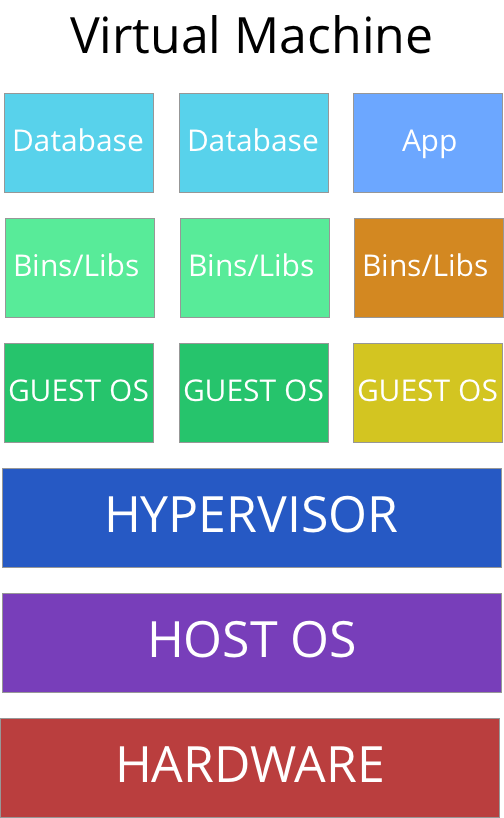
\includegraphics[width=3cm]{img/virtual-machine}
    \caption{structuur van een virtuele machine}
    \label{fig:virtualmachine}
\end{wrapfigure}

Het concept van virtualisatie deelt een aantal gelijkenissen met timesharing. De computer wordt opgedeeld in verschillende delen bij virtualisatie en bij timesharing gaan we de computer opdelen in contexten. De verschillende delen bij beide concepten moeten ook geïsoleerd zijn van elkaar.

Een aantal voordelen van virtualisatie zijn de volgende: financieel voordeel (men kan van één taak naar meerdere taken gaan op één computer), besparen van energie (\cite{beloglazov_energy_2010}) en veiligheid(\cite{mortleman_security_2009}).

Virtuele machines gaan een computer nabootsen. Figuur \ref{fig:virtualmachine} toont de structuur van een virtuele machine. Het laat toe om een besturingssysteem te gebruiken, wanneer de hardware van de fysieke computer dit niet toelaat. Een virtuele machine kan ook de middelen van de fysieke computer waar het zich op bevindt gebruiken. Dit zorgt ervoor dat de middelen van de fysieke computer kunnen gebruikt worden als virtuele middelen. De fysieke computer zal verder naar verwezen worden als de host machine. Guest is de naam dat we geven aan virtuele machines die zich bevinden op de host. In het volgende deel zullen we de laag tussen de host machine en virtuele machine bekijken: de hypervisor. 

\section{Hypervisor}

De hypervisor is een voorbeeld van hardware virtualisatie. Het is een stuk software, firmware of hardware dat de laag vormt tussen de virtuele machine en de host machine. De host machine zorgt voor de middelen zoals CPU, RAM, ... Elke virtuele machine die zich bevindt op de host machine zal dan gebruik maken van een gedeelte van deze middelen. Doordat virtualisatie alomtegenwoordig geworden is in datacenters (\cite{soundararajan_impact_2010}) heeft dit ervoor gezorgd dat er meer logica komt te liggen bij de hypervisor. De hypervisor neemt verder de rol op zich van het verdelen van de middelen en het beheren van de guests. Er zijn twee soorten hypervisors: type 1 en type 2. Type 1 is de bare-metal hypervisor en type 2 de hosted hypervisor. De volgende twee segmenten zullen deze twee verschillende types uitleggen.

\newpage

\subsection{Hosted Hypervisors}

\begin{wrapfigure}{r}{0.3\textwidth}
    \centering
    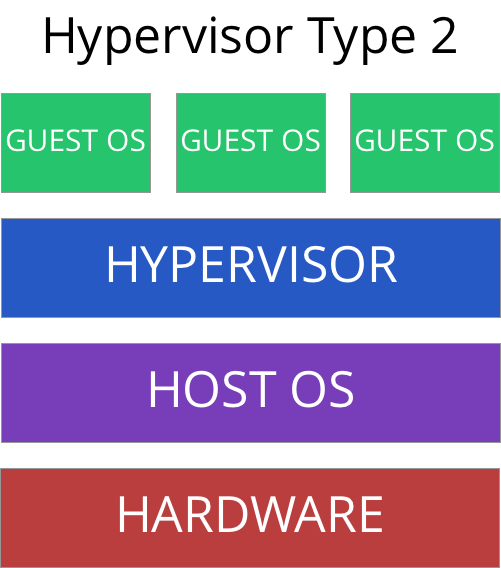
\includegraphics[width=3cm]{img/hypervisor-2}
    \caption{structuur van een hosted hypervisor}
    \label{fig:hypervisor-2}
\end{wrapfigure}

Als eerste zullen we de hosted hypervisor of type 2 hypervisor behandelen. Figuur \ref{fig:hypervisor-2} toont de structuur van een hosted hypervisor. De hosted hypervisor bevindt zich op het besturingssysteem van de host machine en heeft geen directe toegang tot de hardware. Het is wel compleet afhankelijk van het besturingssysteem van de host om zijn taken uit te voeren. Als er problemen optreden in het besturingssysteem van de host zijn er ook problemen bij de hypervisor en daarop volgend de guests. De hele structuur alleen sterk als de host.

Voorbeelden van hosted hypervisors zijn: Oracle Virtualbox (\cite{oracle_oracle_2016}) en VMware Workstation (\cite{vmware_vmware_2016-1}).

\subsection{Bare-metal Hypervisors}

\begin{wrapfigure}{l}{0.3\textwidth}
    \centering
    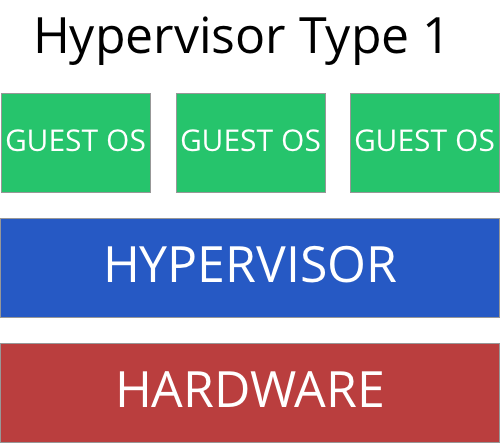
\includegraphics[width=3cm]{img/hypervisor-1}
    \caption{structuur van een bare-metal hypervisor}
    \label{fig:hypervisor-1}
\end{wrapfigure}

Type 1, bare-metal, embedded of native hypervisors bevinden zich rechtstreeks op de hardware. Figuur \ref{fig:hypervisor-1} toont de structuur van een bare-emtal hypervisor. De voornaamste taak van de hypervisor is het beheren en delen van hardware middelen. Dit maakt de hardware hypervisor kleiner in omvang dan de hosted hypervisor. De hypervisor heeft niet het probleem zoals de hosted hypervisor dat er grote problemen kunnen liggen bij het besturingssysteem van de host omdat er geen besturingssysteem is.

Er is een laag minder in de structuur dus dit betekent dat er minder instructies moeten uitgevoerd worden bij een bepaalde handeling en dit geeft een beter performantie. Omdat er geen problemen kunnen zijn met het besturingssysteem van de host kunnen we aannemen dat het stabieler. Wanneer het besturingssysteem van de host faalt bij een hosted hypervisor dan zullen de guests ook falen.

Een paar voorbeelden van bare-metal hypervisors zijn VMware ESXi (\cite{vmware_vmware_2016}) en Xen (\cite{xen_project_xen_2016}).
\section{Operating System-level Virtualization}

Naast hardware virtualisatie kunnen we ook een besturingssysteem virtualiseren. Bij deze toepassing van virtualisatie worden de mogelijkheden van de kernel van het besturingssysteem gebruikt. De kernel van bepaalde besturingssystemen laat toe om meerdere geïsoleerde name spaces tegelijkertijd te laten werken. Dit zorgt ervoor dat de dat er maar één besturingssysteem moet zijn om verschillende programma's naast elkaar en geïsoleerd van elkaar te laten werken.

De verschillende name spaces maken gebruik van CPU, geheugen en netwerk van de host. Elke name space heeft zijn eigen configuratie omdat de user spaces op zichzelf staan en geïsoleerd zijn van de andere user spaces. Dit geeft eveneens de beperking dat guests een besturingssysteem of kernel moeten hebben die overeenkomt met de host.

Tegenover hardware virtualisatie zal besturingssysteem virtualisatie minder gebruik maken van middelen omdat er maar één besturingssysteem is en eveneens het delen van het besturingssysteem. Dit geeft voordelen bij de performantie.

Voorbeelden van besturingssysteem virtualisatie zijn: chroot (\cite{linux_chroot2_????}), Solaris Containers (\cite{oracle_solaris_2016}) en Docker (\cite{docker_docker_2016}).

Besturingssysteem virtualisatie is vooral bekend geworden door Docker vanaf 2013 (\cite{hykes_future_2013}). In het volgende hoofdstuk wordt verder ingegaan op containers en Docker.

\chapter{Containers}
\label{ch:Containers}

\section{Containers}

\begin{wrapfigure}{l}{0.3\textwidth}
    \centering
    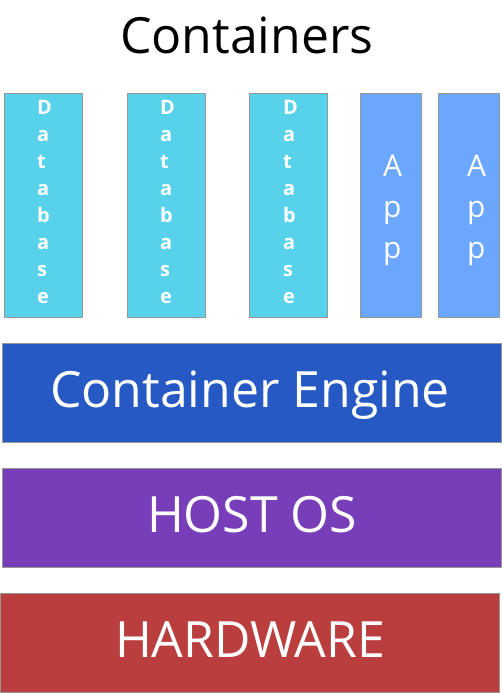
\includegraphics[width=3cm]{img/container}
    \caption{structuur van containers}
    \label{fig:containers}
\end{wrapfigure}

Containers bestaan al een tijd. In \cite{soltesz_container-based_2007} werd al gekeken naar de voordelen van containers tegenover hypervisors. Chroot (\cite{Linux}) is een concept dat veel deelt met containers. Chroot zal de root directory van het huidige proces en zijn children veranderen. Er wordt een virtuele kopie gemaakt van het systeem waarin het proces kan werken. Het proces is dus afgesloten van het systeem en dit zorgt voor meer veiligheid bij het uitvoeren van processen.

Linux Containers of LXC (\cite{containers_linux_????}) is een implementatie van besturingssysteem virtualisatie. LXC kan meerdere geïsoleerde Linux systemen laten werken op één host. Deze geïsoleerde Linux systemen worden containers genoemd. Deze containers worden ook getoond in figuur \ref{fig:containers} waarbij de apps en databases containers zijn. Het volgende deel van deze sectie zal de onderdelen van LXC uitleggen en de voordelen.

Zoals we al gezien hebben is de rol van de hypervisor het delen en beheren van de middelen. Om containers te gebruiken moeten iets anders de rol hiervan overnemen. Cgroups is een Linux kernel extension die deze rol overneemt. Door cgroups kunnen we middelen beheren voor processen tot en met containers. Het toont ook de mogelijkheden om checkpoints te creëren van processen.

Eerder werd ook al aangehaald dat de processen van elkaar gescheiden moeten worden. Dit wordt bereikt door name spaces. De functies die name spaces voorziet zijn uitgebreid. Elke name space heeft zijn eigen file system structure, netwerk interfaces en proces ID space. De containers delen de kernel met alle andere processen die op de kernel aan het werken zijn.

De containers zijn van elkaar afgesloten. Wanneer één container aangetast wordt dan heeft dit geen gevolg op de andere containers.

Toch zijn er een paar andere problemen zoals aangehaald in \cite{madhavapeddy_jitsu:_2015}. Processen die als root werken kunnen niet geïsoleerd worden van elkaar. Verder wordt er ook aangehaald dat strengere isolatie nodig is. (tabel 2, \cite{madhavapeddy_jitsu:_2015})

\section{Docker}

Het was een kwestie van tijd dat de puzzelstukken in elkaar vielen. Dit gebeurde met Docker (\cite{docker_docker_2016}). 

Docker was het bedrijf dat al de delen samenbracht onder uitgebreid ecosysteem. Docker maakte de handelingen rond containers simpeler en intuïtief. Het werd gemakkelijk om containers te maken en te delen met andere. Door veel van de componenten van het ecosysteem open te stellen konden ze rekenen op de steun van vele ontwikkelaars.

Er waren andere formaten dan Docker zoals Rocket die het mogelijk maakte voor containers te maken. Maar door hun ecosysteem en de hulp van de open source gemeenschap hebben is Docker de standaard geworden om containers te maken en ermee te werken.

In 2015 werd het Open Container Initiative opgericht. Veel van de grote spelers op vlak van containers zoals Docker, CoreOS, Microsoft en Google maken hier deel van uit. Ze willen een standaard voor containers vastleggen.

In het volgende hoofdstuk bekijken we de werking en mogelijkheden met unikernels.

\chapter{Unikernels}
\label{ch:unikernels}

\section{Inleiding}

Dit hoofdstuk zal uitleggen waarom unikernels ontwikkeld worden. De verschillende eigenschappen en voordelen worden ook aangehaald. Als laatste deel van dit hoofdstuk wordt bekeken welke implementaties van unikernels er al bestaan en wat de verschillende ertussen zijn.

Virtuele machines (hoofdstuk \ref{ch:virtualisatie}) zijn er gekomen wanneer men de middelen van computers beter wou gebruiken. Toch werden de middelen niet ten volle gebruikt door grote besturingssystemen met enkele werkende processen. Maar er zijn processen die aan het werken zijn maar geen nut hebben. Containers (hoofdstuk \ref{ch:Containers}) waren een reactie op dit probleem. De middelen werden efficiënter gebruikt doordat er maar één besturingssysteem was en de containers de delen van het host OS hergebruikten. De isolatie en veiligheid van containers zorgt wel voor een aantal problemen. Unikernels probeert het probleem van veiligheid en isolatie op te lossen en de voordelen van containers te behouden.

De eerste implementaties van unikernels komen we tegen op het einde van de jaren 90. Exokernel (\cite{mit_mit_1998}) werd ontwikkelt door MIT. Het had als doel zo weinig mogelijk abstractie de software ontwikkelaars op te leggen. De software ontwikkelaars kunnen zelf keuzes maken voor de abstractie. Nemesis (\cite{university_of_cambridge_nemesis_2000}) werd vanuit University of Cambridge ontwikkeld. Ze hadden eerder multimedia use cases als doel in hun achterhoofd.

Unikernels vragen inzicht in een aantal verschillende concepten. De kernel ligt aan de basis van een besturingssysteem en zal in de volgende sectie worden uitgelegd.

\section{Kernel}

De kernel is het programma dat zich centraal bevindt in het besturingssysteem. Het werkt rechtstreeks met de hardware van de computer. De kernel kan gezien worden als het fundament waar het hele besturingssysteem op steunt. Omdat het een belangrijke rol vervult in de computer is veel van het geheugen van de kernel beveiligd zodat andere applicaties geen veranderingen kunnen aanbrengen. Als er iets fout zou gaan met de kernel, dan heeft dit rechtstreeks gevolgen op het besturingssysteem. Al de handelingen die de kernel uitvoert bevinden zich in de kernel space. Daartegenover gebeurd wat de gebruiker uitvoert in de user space. Het is van uiterst belang dat de kernel space en user space strikt van elkaar gescheiden zijn. Als dit niet zo zou zijn dan zou een besturingssysteem en tevens de computer onstabiel en niet veilig zijn. De kernel voert nog andere taken uit zoals memory management en system calls. Figuur \ref{fig:kernel} toont de positie van de kernel aan.

\begin{wrapfigure}{r}{0.3\textwidth}
    \centering
    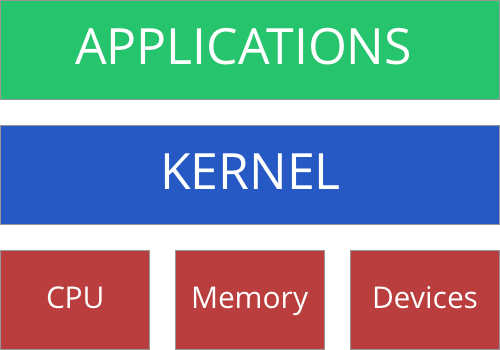
\includegraphics[width=3cm]{img/kernel}
    \caption{positie van kernel tussen de programma's en hardware}
    \label{fig:kernel}
\end{wrapfigure}

Als een programma wordt uitgevoerd dan bevindt die zich in de user space. Om het programma in werkelijkheid te kunnen uitvoeren moet toestemming gevraagd worden aan de kernel om de instructies van het programma realiseren. Deze instructies moeten worden nagegaan voor de veiligheid. Soms wordt er ook gesproken van memory isolation, waarbij de user space en kernel space niet rechtstreeks met elkaar kunnen communiceren. Dit is een veiligheidsmaatregel.

Volgend boek heeft meer informatie over de werking van de kernel (\cite{bovet_understanding_2005}).

De twee volgende delen van library besturingssysteem en single address space dat hierop volgt, zal de twee belangrijkste eigenschappen van unikernels uitleggen.

\section{Library besturingssysteem}

Elke virtuele machine binnen de architectuur van cloud computing heeft meestal één functie. Dit is al getoond in figuur \ref{fig:virtualmachine}. Elke guest heeft een gespecialiseerde rol om de middelen dat het ter beschikking krijgt optimaal te benutten.
Dezelfde architectuur van kan men terugvinden bij containers. De besturingssystemen die de virtuele machines en containers gebruiken is algemeen te noemen. Dit is aangehaald in \cite{madhavapeddy_unikernels_2013}.

Als er dieper wordt ingegaan op deze evolutie dan wordt er vastgesteld dat er steeds kleinere eenheden worden gebruikt. Eerst was de computer de eenheid, dan werd er van virtuele machine naar containers gegaan.

Het meest gebruikte besturingssysteem voor servers is het Ubuntu besturingssysteem (\cite{matthias_gelbmann_ubuntu_2016}) met 32\%. Veel programma's van databases tot en met web applicaties gebruiken het. Dit terwijl een database en een web applicatie andere middelen en functies nodig hebben.
Er zijn er ook gespecialiseerde besturingssystemen zoals Mini-OS (\cite{satya_popuri_tour_????}) die veel van de overbodige functies van een algemeen besturingssysteem niet gebruiken. Deze gespecialiseerde besturingssystemen zijn wel in de minderheid.

Algemene besturingssystemen zijn niet de basis die men nodig heeft in een architectuur waar elke eenheid gespecialiseerd is. Alpine (\cite{alpine_linux_development_team_alpine_????}) is een Linux besturingssysteem dat zeer minimaal is. Het beschikt over een uitgebreide package repository. Dit maakt het een ideaal besturingssysteem voor containers mee te bouwen. Je kan starten met een kleine basis en alle onderdelen toevoegen die je nodig hebt. Dit zorgt voor betere performantie en een container met kleinere omvang.

\begin{wrapfigure}{r}{0.4\textwidth}
    \centering
    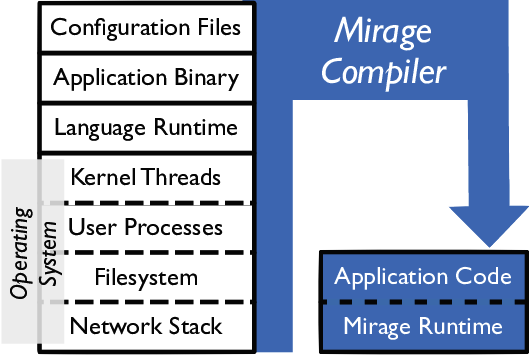
\includegraphics[width=6cm]{img/unikernel}
    \caption{algemeen besturingssysteem tegenover een unikernel implementatie \cite{madhavapeddy_unikernels_2013}}
    \label{fig:unikernel}
\end{wrapfigure}

Niet alleen hebben sommige delen geen nut meer, maar soms kan dat ervoor zorgen dat de performantie van een besturingssysteem gehinderd wordt voor bepaalde taken. Het is dezelfde analogie als het gebruiken van een hamer voor elke klus.

Alpine is zeer miniem als besturingssysteem. Het concept van Library besturingssysteem (\cite{madhavapeddy_unikernels_2013}) neemt dit nog een stap verder. Er wordt met een absoluut minieme basis gestart. Daarna worden alleen de componenten toegevoegd die nodig zijn voor de functie die de eenheid uitvoerd. Library duidt op de verschillende onderdelen of componenten die je kan toevoegen.

Web applicaties hebben verschillende functies nodig om te kunnen communiceren. Hiervoor bestaan netwerkprotocollen. TCP is een kritiek protocol om te communiceren met internet. Bij algemene besturingssystemen, zoals Ubuntu, is dit al aanwezig. Omdat er gestart wordt met een minimale basis, moeten deze protocollen geïmplementeerd worden. Gelukkig zijn er libraries die hiervoor kunnen gebruikt worden. De libraries, broncode en configuratie worden dan gecompileerd. Als resultaat heb je dan een afbeelding. Deze afbeelding wordt een unikernel genoemd. De unikernel wordt gecompileerd voor één omgeving en kan alleen gebruikt worden op die omgeving. Dit is een verschil met containers en virtuele machines die meer los staan van de omgeving dan unikernels.

Er werd al gesproken dat de unikernel alleen zal werken op de omgeving waarvoor het gecompileerd is. Dit is omdat de drivers voor de hardware componenten moeten worden geschreven. Kleine veranderingen in de specificatie of interface van een hardware component zorgt ervoor dat de driver niet meer werkt. Drivers zijn de grootste hindering die men tegenkomt bij library besturingssystemen. Hypervisors lossen dit probleem op door een standaard interface open te stellen. Zo moet er alleen maar één driver worden geschreven voor de hardware component. Dit neemt veel van het werk voor het maken van unikernels weg. De protocollen waar eerder over gesproken is het grootste werk bij unikernels.

Een unikernel wordt bekeken als een eenheid.

\section{Single Address Space}

In een unikernel bestaat er geen concept van user of kernel space. Alle processen bevinden zich in dezelfde omgeving. Dit zou problemen geven bij traditionele besturingssystemen. Maar bij het compileren van de unikernel wordt de broncode, libraries en configuratie gecontroleerd. Dit is om te kijken of er zich geen problemen kunnen voordoen. De afwezigheid van het vragen van toestemming tussen de twee spaces zorgt voor betere performantie. Deze verbetering van performantie komt doordat de hardware kan worden aangesproken zonder dat er verandert moet worden van context.

Eén globale address space zorgt voor problemen met de isolatie van processen. Meerdere programma's naast elkaar laten werken op een library operating system is complex. De hypervisor lost dit probleem gedeeltelijk op. Een mogelijke oplossing voor dit probleem wordt verder besproken in Hoofdstuk \ref{ch:architectuur-met-unikernels}.

\section{Veiligheid}

De hoge veiligheid van unikernels is een gevolg van de specialisatie van de eenheid. Bij virtuele machines en containers zijn algemene besturingssystemen de basis. Deze besturingssystemen hebben zeer veel functionaliteit dat niet nodig is voor de taak dat ze uitvoeren. De overbodige functionaliteit kan zorgen voor een lagere performantie, maar ook voor meer veiligheidsrisico's. Het is gemakkelijker om de veiligheid te garanderen van een kleine codebasis tegenover een grote. Daar komt nog bij dat er specifieke implementaties zijn voor een omgeving. Het is veel moeilijker om zelf code te schrijven voor een specifieke implementatie te buiten tegenover een algemene implementatie.

Verder heeft een unikernel geen shell of een andere mogelijkheid om een unikernel aan te passen terwijl hij aan het werken is. Eén unikernel overnemen heeft geen gevolg op de andere unikernels. Daarbij komt nog dat hypervisors meer veiligheid garanderen (\cite{colp_breaking_2011}).

\section{Andere voordelen}

De omvang van een unikernel is zeer laag tegenover een virtuele machine of een container. Zoals we al eerder aanhaalden kunnen containers ook zeer klein zijn wanneer ze een miniem besturingssysteem gebruiken. Een voorbeeld daarvan is Alpine dat start vanaf 5 MB (\cite{_gliderlabs/docker-alpine_????}).
Een voorbeeld van de omvang van een unikernel kan gevonden worden in \cite[hoofdstuk 4, p.~10]{madhavapeddy_jitsu:_2015} met 1 MB.

Het systeem optimaliseren kan ook in veel grotere mate gebeuren (\cite{madhavapeddy_turning_2010}) dan algemene besturingssystemen.

\section{Productie}

Veel van het commentaar op unikernels komt van de moeilijkheid om te kijken wat er fout gaat in productie (\cite{bryan_cantrill_unikernels_2016}). Aanpassingen doen in productie om problemen te verhelpen is niet de beste manier om iets op te lossen. Het programma moet uitgebreid getest worden vooraleer het productie wordt opgesteld. Wanneer er dan toch iets fout gaat in productie dan zal men de situatie proberen na te bootsen in een soortgelijke omgeving. Het terugzetten van een oudere versie van de applicatie kan helpen om de gebruikers geen ongemak te voorzien en tevens meer tijd te hebben om bepaalde problemen op te lossen.

\section{Hedendaags gebruik}

Unikernels kunnen momenteel gebruikt worden in uiterst bepaalde situaties. Er was hetzelfde fenomeen bij containers een paar jaar geleden vooraleer Docker op de voorgrond trad. Elke technologie zal dit ondergaan omdat iets intuïtiever maken en veralgemenen kost tijd.

In het volgende deel zullen we implementaties van unikernels vergelijken om een beeld te krijgen van de huidige mogelijkheden.

\chapter{Vergelijking implementaties unikernels}

\section{Inleiding}

In het hoofdstuk over unikernels zijn er een aantal voorbeelde van moderne implemenaties van unikernels aangehaald. Hierbij zijn er verschillende criteria die aangehaald kunnen worden. In volgende sectie zullen we de criteria beschrijven.

\section{Criteria}

\begin{description}
\item [Implementatie programmeertaal]
In welke programmeertaal is de implementatie geschreven? De meeste implementaties zijn in C/C++ geschreven. Dit komt vooral door het feit dat veel software ontwikkelaars die zich bezig houden met unikernels komen vanuit een achtergrond met besturingssystemen komen.
De meest gebruikte programmeertaal voor een besturingssysteem is C/C++.

\item [Hypervisors] 
Hypervisors zijn een groot deel waarom unikernels gekozen worden. De meest gebruikte unikernels zijn beschikbaar op een aantal hypervisors. Sommige unikernels specialiseren zich in één hypervisor.
Dit is om gebruik te maken van de specifieke mogelijkheden van de hypervisor en zo de sterktes daarvan uit te buiten.

\item [Ondersteunde programmeertalen] 
De grootste factor bij het kiezen van een implementatie van een unikernel. Het is gemakkelijker om een bepaalde implementatie te gebruiken wanneer je kan kiezen uit een aantal programmeertalen.
Als je een microservice wilt schrijven in een andere programmeertaal, zou het wel handig ze om bij dezelfde implementatie te blijven.

\item [GitHub stars] 
Hieruit kunnen we opmaken hoeveel mensen het in de gaten houden en hoe populair is.

\end{description}

{\footnotesize
\begin{center}
    \begin{tabular}{| l | l | l | l | l |}
    \hline
    Naam & Taal implementatie & Hypervisor & Ondersteunde talen & GitHub sterren \\ \hline
    ClickOS & C/C++ & Xen & bindings & 243 \\ \hline
    HaLVM & Haskell & Xen & Haskell & 665 \\ \hline
    LING & C/Erlang & Xen & Erlang & 523 \\ \hline
    Rumprun & C & hw, Xen, POSIX & C, C++, Erlang, Go, ... & 469 \\ \hline
    MirageOS & OCaml & Xen & OCaml & 657 \\ \hline
    IncludeOS & C++ & KVM, VirtualBox & C++ & 1341 \\ \hline
    OSv & C/C++ & KVM, Xen, ... & JVM & 2121 \\ \hline
    \end{tabular}
\end{center} 
}

De inhoud van de bovenstaande tabel wordt per implementatie uitgelegd in het volgende deel.

\newpage

\section{Implementaties van moderne unikernels}

\subsection{ClickOS (\cite{martins_clickos_2014})}
\begin{description}
  \item [Implementatie programmeertaal]: C/C++
  \item [Hypervisors]: Xen
  \item [Ondersteunde programmeertaal]: ondersteund door bindings
  \item [GitHub stars]: 243
\end{description}

Deze implementatie van een unikernel wordt ontwikkeld door Cloud Networking Performance Lab.

De programma's waarvoor ClickOS wordt voor gebruikt zijn middleboxes. Een middlebox is een netwerk applicatie dat netwerktrafiek kan omzetten, filteren, inspecteren of manipuleren. Voorbeelden hiervan zijn firewalls en load balanceres.
Een modulaire software vormt het startpunt. Op de router worden onderdelen toegevoegd. Deze unikernel werkt alleen op MiniOS. MiniOS is beschikbaar bij de source van de Xen hypervisor.

Door een evolutie binnen netwerk laag (\cite{garcia_villalba_trends_2015}) wordt veel van de functionaliteit, die vroeger bij de hardware zat, nu in software geïmplementeerd. Dit laat het toe om een eigen implementatie schrijven om veel van functionaliteit van de hardware over te nemen.
Dit zorgt voor een implementatie die aangepast kan worden aan de eigen situatie.

De use cases waarbinnen ClickOS kan gebruikt worden zijn beperkt. Als je geen gebruik wilt maken van ingebouwde netwerk functionaliteit van de hardware dan is ClickOS de uitgesproken keuze.

Er wordt Swig gebruikt om ondersteuning te bieden voor hogere programmeertalen. Swig maakt een bindings die C/C++ verbindt met een hogere taal.

ClickOS verwijst naar zijn packages als elements. Die elements voeren in bepaalde actie uit. Dit zijn hele kleine stukken functionaliteit. Er zijn om en bij de 300 elementen aanwezig. Het is niet moeilijk om zelf je element te maken.

Meer informatie kan gevonden worden op \cite{cloud_networking_performance_lab_cloud_????}.

\subsection{HaLVM (\cite{galois_inc._haskell_????})}

\begin{description}
  \item [Implementatie programmeertaal]: Haskell
  \item [Hypervisors]: Xen
  \item [Ondersteunde programmeertaal]: Haskell
  \item [GitHub stars]: 665
\end{description}

HaLVM wordt ontwikkeld door Galios. Galios is software development agency dat unikernels al een tijd in productie gebruikt.
Er zijn niet veel bedrijven die unikernels al gebruiken in productie, dus ze hebben veel ervaring met de mogelijkheden en moeilijkheden van unikernels.

De programmeertaal waarin de unikernel van HaLVM wordt geschreven is Haskell. Haskell is een functionele programmeertaal met een uitgebreid type system. HaLVM is een specifieke implementatie die één supervisor en programmeertaal ondersteund.

Het werd ontwikkeld met als doel voor besturingssysteem componenten snel te maken en te testen. Maar na een tijd is het geëvolueerd naar andere use cases.

Bij HalVM wordt de Xen hypervisor als omgeving gebruiken. Er is een integratie met de Xen hypervisor waarop de core library van HaLVM op rust. Er bestaat ook een communications library die bestaat uit Haskell File System en Haskell Network Stack. Deze library kan gebruikt worden in de meeste gevallen als je een netwerkfunctionaliteit nodig hebt. Als we meer mogelijkheden nodig hebben voor de applicatie dan gaan we modules toevoegen. Er is een ecosysteem uitgebouwd om het gemakkelijker te maken voor software ontwikkelaars om hun eigen modules te bouwen.

De werkwijze is de volgende: eerst wordt er zoveel mogelijk functionaliteit als een normaal Haskell programman geschreven. Daarna moet het programma beginnen aangepast worden om het te gebruiken op HaLVM.
Dit is niet gemakkelijk bij uitgebreide applicaties zijn, want er zijn maar beperkte mogelijkheden om te debuggen op HalVM.

Zoals in de meeste gevallen moet de compiler van Haskell worden aangepast om rechtstreeks te kunnen werken op de Xen hypervisor. Het is ook geen probleem om standaard Haskell libraries in de code te gebruiken.

Het wordt gebruikt door Galios in productie en dit maakt het gemakkelijk om vragen te stellen. De GitHub repository waar de applicatie zich op bevindt, is over het algemeen actief.

\subsection{Ling (\cite{erlang_on_xen_cloudozer/ling_????})}

\begin{description}
  \item [Implementatie programmeertaal]: C/Erlang
  \item [Hypervisors]: Xen
  \item [Ondersteunde programmeertaal]: Erlang
  \item [GitHub stars]: 523
\end{description}

Ling is een Erlang virtuele machine die werkt op Xen. Het bedrijf achter Ling is Cloudozer. Ze hebben al meerdere language runtimes gemaakt die rechtstreeks op Xen werken.
Ling is open source maar de andere tools, die het beheren doen, zijn niet open source. Wanneer je problemen met het ecosysteem moet de ondersteuning van Cloudozer gecontacteerd worden.

Zoals bij HaLVM moet eerst de applicatie geschreven worden in Erlang. De package manager die gebruikt word met Erlang is Rebar, dit is de standaard Erlang package manager. Na het omzetten van de applicatie naar een Xen afbeelding zou de unikernel moeten werken.

Railing is een tool die meegeleverd is met Ling die je toelaat om erlang on Xen afbeeldingen te maken. We gebruiken ook xl utility van Xen om domeinen te beheren.
De focus van Erlang on Xen was de Xen hypervisor in het begin. Met het uitbrengen van LING is het mogelijk geworden om ports te maken voor andere omgevingen. Dit heeft veel nieuwe omgevingen voor IOT en mobiele applicaties mogelijk gemaakt.
Unikernel kunnen handig zijn op deze omgevingen omwille van de kleine omvang. Verder opent dit ook de mogelijkheid voor de unikernels van LING op bare-metal te laten werken.

\subsection{Rumprun (\cite{rumpkernel/rumprun_0000})}

\begin{description}
  \item [Implementatie programmeertaal]: C
  \item [Hypervisors]: hardware, Xen, KVM
  \item [Ondersteunde programmeertaal]: onder meer C, C++, Erlang, Go, Javascipt, Python, Ruby
  \item [GitHub stars]: 469
\end{description}

Rumprun gebruikt rump kernels voor hun implementatie. Deze rump kernels worden samengesteld uit componenten afkomstig van NetBSD. NetBSD is een algemeen besturingssysteem maar is modulair geschreven.
Men kan het dus gebruiken om een rump kernel te samen te stellen. De rump kernel wordt dan samen met de applicatie verpakt om gebruikt te kunnen worden in verschillende omgevingen.

Er is een uitgebreide collectie van hypervisors waaruit je kan kiezen wanneer je een rumprun applicatie hebt. De term hw duidt op hardware. Dit betekent dat rumprun één van de enige implementaties is die rechtstreeks kan werken op hardware. De unikernel kan ook werken op besturingssystemen die een POSIX-interface hebben.

Er zijn verschillende soorten unikernels. Sommige unikernels specialiseren op basis van programmeertaal en andere op basis van omgeving. Sommige doen zelf beide. Rumprun doet beide. Dit is wel niet zonder gevolg. De performantie zal niet een gespecialiseerde unikernel kunnen evenaren.

Er wordt ook aangehaald in de wiki dat wanneer een programma de mogelijkheid heeft om een gespecialiseerde unikernel te gebruiken, gebruik je best die oplossing. Als dit niet het geval is dan kan een rumprun kernel een goede oplossing zijn.

De rump-run packages zijn implementaties van drivers, protocollen en libraries die kunnen toegevoegd worden aan rumprun kernels. Er zijn een groot aantal packages die kunnen gebruikt en de meest bekende zijn zeker aanwezig.
Het spijtige is wel dat er nog geen packaging systeem aanwezig is. Dit zou er wel voor zorgen dat er gewerkt kan worden met verschillende dependencies en versies van packages.

Rumprun verziet zelf geen compiler. Er wordt gebruik gemaakt van een compiler die aanwezig is op het systeem. In het geval van Mac OS X moet je een aparte compiler installeren. Het is wel goed dat native op Mac OS X de build tools kunnen gebruikt worden. Meestal moet je zelf een omgeving opstellen.

De programmeertalen die ondersteund zijn, zijn de volgende: C, C++, Erlang, Go, Javascript(node.js), Python, Ruby en Rust. De keuze van programmeertalen is uitgebreid.

Meer informatie is te vinden in volgende thesis: \cite{kantee_flexible_2012}.

\subsection{MirageOS (\cite{mirage/mirage_0000})}

\begin{description}
  \item [Implementatie programmeertaal]: OCaml
  \item [Hypervisors]: Xen, Unix
  \item [Ondersteunde programmeertaal]: OCaml
  \item [GitHub stars]: 657
\end{description}

Er kan gezegd worden dat het voor een deel allemaal begon bij MirageOS. Hun paper (\cite{madhavapeddy_unikernels_2013}) over unikernels en MirageOS wakkerde veel interesse aan rond unikernels. Ervoor was er wel al sprake van unikernels maar MirageOS zorgde voor veel nieuwe initiatieven.

Mirage is een cloud besturingssysteem gemaakt voor veilige netwerk applicaties met een hoge performantie te maken op verschillende omgevingen.

De programmeertaal dat gebruikt word voor een MirageOS applicatie te maken is OCaml.
OCaml is de algemene implementatie van de Caml programmeertaal en voegt object georiënteerd programmeren toe. Het wordt extensief gebruikt door facebook. Deze taal is niet heel erg bekend en dit kan ervoor zorgen dat het niet veel tractie heeft.
De voornaamste redenen om OCaml te gebruiken zijn static type checking en automatic memory management. De eerste reden is om tegen te gaan dat er iets fout gaat wanneer een applicatie aan het werken is. De compiler gaat kijken of hij geen onveilige code kan vinden. Als dit het geval is, wordt er het programma niet gecompileerd.
Memory management is belangrijk voor resource leaks tegen te gaan. Resource leaks kunnen ervoor zorgen dat de applicatie meer resources gebruikt dan nodig is of zelf het programma of systeem laten stoppen met werken.

De applicatie kan geschreven worden op een Linux of Mac OSX machine. Deze applicatie kan dan werken op een Xen of Unix omgeving. Dit geeft veel mogelijkheden voor het te gebruiken.

MirageOS bestaat al een tijd en heeft een groot aantal libraries ter beschikking. Het heeft een uitstekende toolchain voor het compileren van applicaties en het debuggen van de resulterende unikernel. Debuggen kan soms tot problemen leiden bij unikernels want men kan niet zelf in de unikernel kijken. Dit komt omdat de unikernel geen shell heeft. De debug optie kan hierbij helpen. De resulterende unikernel kan ook werken op mobiele omgevingen.

\subsection{IncludeOS (\cite{oslo_and_akershus_university_college_hioa-cs/includeos_????})}
\begin{description}
  \item [Implementatie programmeertaal]: C/C++
  \item [Hypervisors]: KVM, VirtualBox
  \item [Ondersteunde programmeertaal]: C++
  \item [GitHub stars]: 1341
\end{description}

IncludeOS is gemotiveerd door \cite{bratterud_maximizing_2013}. Het onderscheid tussen een minimale virtuele machine tegenover een unikernel is zeer klein. Daarom worden beide termen afwisselend gebruikt. Net zoals ClickOS moeten de applicaties geschreven worden in C++.

IncludeOS zorgt voor een bootloader, standaard libraries, modules voor drivers te implementeren en een build- en deploysysteem. Het is simpel om applicaties te maken voor deze unikernel. Je moet allen één dependency toevoegen aan het programma. Dan kan het worden omgezet naar een unikernel. Er veranderd dus niet veel voor de developers zelf. Dit zorgt voor een vlotte overgang en is zeker belangrijk wanneer men kiest voor minimale applicaties te maken.

Meerdere processen tegelijk laten werken op een unikernel van includeOS is niet mogelijk. Dit kan sommige software ontwikkelaars afschrikken. Het gebruik van microservices (hoofdstuk \ref{ch:architectuur-met-unikernels} sectie \ref{ch:microservices}) is nog niet wijdverspreid en kan een factor zijn bij het selecteren van een unikernel implementatie. Enerzijds gaan bedrijven nooit bij unikernels komen wanneer hun architectuur niet gebaseerd op microservices. Er zijn ook geen race conditions mogelijk omdat er maar één proces mogelijk is.

Momenteel ligt de focus van IncludeOS voornamelijk op C++. Dit is een strategie dat kan helpen wanneer software ontwikkelaars zoeken naar een implementatie die een gemeenschap heeft. IncludeOS heeft een grote gemeenschap van C++ software ontwikkelaars. Hun doel is vooral om een soortgelijk Node.js te maken maar dan in efficiënt C++.

Er zijn geen plannen om hogere programmeertalen zoals Javascript te ondersteunen. Ook is IncludeOS niet POSIX compliant en dit kan voor problemen zorgen wanneer er extra functionaliteit moet worden toegevoegd.

Als omgeving focussen ze KVM en virtualbox. Hier is het dus gemakkelijk om een unikernel te testen op je eigen machine. Als je services schrijft in C++ dan is IncludeOS een zeer goede keuze. Er kan meer informatie gevonden worden op de GitHub repository: \cite{oslo_and_akershus_university_college_hioa-cs/includeos_????}.

\subsection{OSv (\cite{cloudius-systems/osv_0000})}

\begin{description}
  \item [Implementatie programmeertaal]: C/C++
  \item [Hypervisors]: VMWare, VirtualBox, KVM, Xen
  \item [Ondersteunde programmeertaal]: Java
  \item [GitHub stars]: 2121
\end{description}

De meest uitgebreide unikernel vanuit mijn oogpunt is OSv. Er wordt een hoog aantal programmeertalen geondersteund. Waaronder Java, Ruby, Javascript, Scala en vele anderen. Hierbij moeten wel wel vermelden dat de implementaties van Ruby en Javascript in Java zijn geschreven. Rhino en JRuby zijn de namen hiervan. Het is simpel om deze programmeertalen toe te voegen wanneer je Java als taal al ondersteunt. Er wordt gewerkt aan de native ondersteuning voor deze talen.

Verder kunnen de resulterende unikernels werken op veel omgevingen: VMware, VirtualBox, KVM en Xen. Het is een indrukwekkende lijst van hypervisors de je kan gebruiken. Dit kan helpen om tegen te gaan dat men vast zou zitten op een bepaalde omgevingen.

Zoals IncludeOS voorheen is OSv geschreven in C++.

Voor het beheren van een OSv instance kan gebruik worden gemaakt van de GUI. Bij de meerderheid van unikernels is informatie te vinden door middel van een GUI onmogelijk. Extensies met de hypervisor kunnen hierbij helpen, maar dan nog laat de UX de wensen over. De GUI is gebouwd op een REST API die de componenten van OSv openstellen. Dit komt overheen met de manier hoe docker hun architectuur werkt. Deze componenten stellen een API open waar de tools verder opgebouwd kunnen worden. Er is een API-specificatie die lokaal kan bekeken worden.

OSv ondersteund Amazon Web Services en Google Container Engine als cloud providers. Het is uitzonderlijk dat een unikernel zoveel informatie heeft over hoe het moet gebruikt worden. Er is documentatie over cloud providers, hypervisors, hoe OSv moet gebruikt worden, hoe programma's moet omgezet naar de implementatie. En wat nodig is om zelf te sleutelen aan OSv.

Het is de meest populaire implemenatie van unikernels van alle implementaties die we hebben overlopen op GitHub. Ook de activiteit op de Github repository is het hoogste.

Meer informatie is te vinden in volgende paper: \cite{kivity_osvoptimizing_2014}.

\section{Conclusie}

Er zijn veel verschillende soorten implementaties van unikernels op dit moment. Er is MirageOS die als één van de eerste opkwam en ook de meest extreme weg opgaat met het starten van een minieme basis. HalVM bevindt zich in aan de dezelfde kant als MirageOS. Terwijl OSv en Rumprun zich bevinden aan de overkant. Ze ondersteunen een groot aantal programmeertalen en omgevingen. Dit wordt mogelijk gemaakt door een compatibel laag te gebruiken. 

Hetzelfde fenomeen kunnen we vinden met de toepassingen waar de unikernels kunnen voor gebruikt worden. ClickOS heeft vooral middlebox applicaties als doel en andere unikernels kunnen voor uiteenlopende situaties kunnen gebruikt worden.

\chapter{Architectuur in een wereld van unikernels}
\label{ch:architectuur-met-unikernels}

\section{Microservices}
\label{ch:microservices}

Over het algemeen worden programma's gemaakt als één grote blok. Al de functionaliteit en verantwoordelijk wordt gestopt in één programma. Een programma veel afzonderlijke functionaliteit bezit, noemen we een monoliet of monolith in het Engels. De architectuur waarin deze soort applicaties voorkomen noemen we een monolithische architectuur. Software ontwikkelaars worden geleerd door middel van patronen om functionaliteit en verantwoordelijkheid van elkaar te scheiden. Modulariteit is hierbij een belangrijk gegeven.

\begin{wrapfigure}{r}{0.4\textwidth}
    \centering
    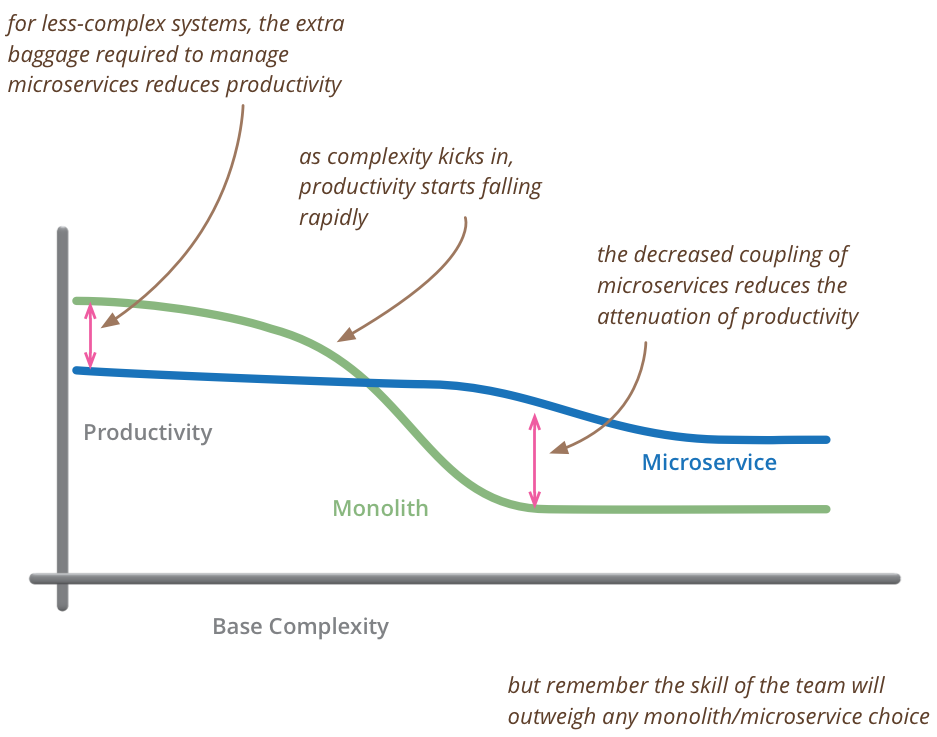
\includegraphics[width=6cm]{img/microservices_monolith}
    \caption{Productiviteit en complexiteit van microservices architectuur tegenover een monolithische architectuur (\cite{martin_fowler_microservicepremium_2015})}
    \label{fig:pr}
\end{wrapfigure}

Een probleem dat veel voorkomt bij een monolithische architectuur is dat het programma zeer complex wordt na een tijd. Functionaliteit toevoegen is niet vanzelfsprekend meer. Er moet rekening worden gehouden met de andere delen van het programma. Nieuwe ontwikkelaars die het programma niet kennen moeten eerst een paar weken het programma verkennen. Dan pas kan er begonnen worden met nieuwe functionaliteit te schrijven.

Schaalbaarheid is een probleem waar ook tegen gelopen wordt na een tijd. Sommige onderdelen van een programma moeten meer trafiek kunnen verwerken dan andere delen. Zoals we al aanhaalden in hoofdstuk \ref{ch:virtualisatie}. Sommige programma's hebben nu éénmaal een andere verdeling van middelen nodig. Dit is hetzelfde bij de interne delen van programma. Het schalen van deze componenten is alleen mogelijk door een nieuwe instantie toe te voegen van de hele applicatie of de implementatie te verbeteren.

Al langer bestaat het idee om een groot programma op te splitsen in kleinere programma's. Telecommunicatie is een industrie waarin microservices al werden gebruikt \cite{griffin_survey_2007}. De opkomst van containers heeft dit idee alleen maar meer verspreid. De architectuur waarbinnen dit idee wordt gebruikt, wordt microservices architectuur genoemd. De microservices kunnen we bekijken als deelapplicaties die één verantwoordelijkheid hebben.

\begin{wrapfigure}{r}{0.4\textwidth}
    \centering
    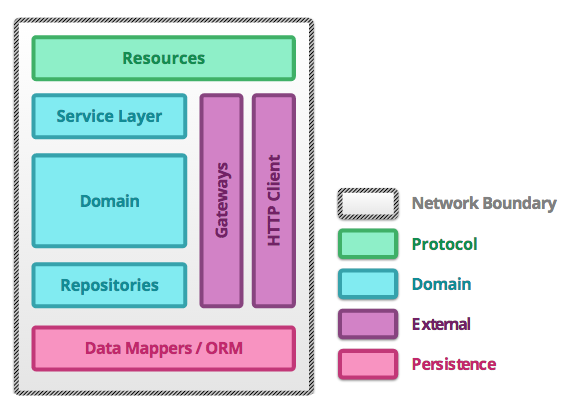
\includegraphics[width=6cm]{img/microservice_structure_example}
    \caption{Structuur van een architectuur met microservices (\cite{toby_clemson_testing_2014}) }
    \label{fig:microservice_structure_example}
\end{wrapfigure}


Een programma opsplitsen in componenten, met één verantwoordelijkheid, zorgt ervoor dat het meer schaalbaar is. Containers en unikernels helpen hierbij. Het opstarten van een nieuwe instantie van een microservice neemt minder tijd in beslag dan een nieuwe instantie dan een monoliet.

Bij microservices zal de topologie van het probleem moeten gekend zijn. Starten met het gebruiken van microservices architecture wanneer men het domein niet goed kent, vraagt om problemen. Het ontwerpen van een microservices architectuur moet goed uitgewerkt zijn. Anders kan later gelopen worden op problemen met de architectuur. Een monolithische architecture zal beter kunnen reageren op dit probleem. Als men later het domein kent kunnen we een microservices architecture gebruiken. Hiervoor moet men de monoliet modulair schrijven. Modulairiteit is een vanzelfsprekende bouwsteen binnen programmeren dus we kunnen hiervan uitgaan.

De complexiteit van een monoliet wordt overgebracht naar het communiceren en het behouden van de consistentie van de microservices. Verder wordt ook het opstellen de architectuur moeilijker. Dit betekent dat er meer werk komt te liggen bij systeembeheerders.

Het voordeel van een microservices architecuur is dat de microservices van elkaar gescheiden zijn. Het gebruik van een nieuwe technologie of framework is niet een groot probleem meer, omdat de microservices los van elkaar staan. Er kan dus een andere programmeertaal gebruikt worden zolang de communicatie tussen de microservices consistent blijft.

De communicatie van de microservices gebeurd via het netwerk. Dit maakt het mogelijk om microservices op verschillende virtuele machines of containers te laten werken. Het concept van software defined network (\cite{garcia_villalba_trends_2015}) neemt veel complexiteit weg van de communicatie.

\begin{wrapfigure}{r}{0.4\textwidth}
    \centering
    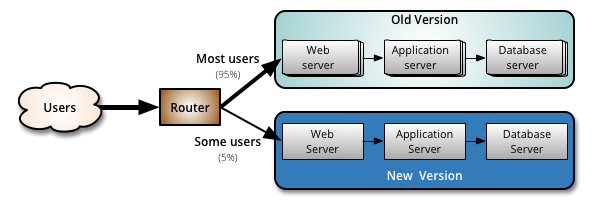
\includegraphics[width=6cm]{img/canary-release}
    \caption{Voorbeeld van een canary release (\cite{danilo_sato_canaryrelease_2014})}
    \label{fig:canary-release}
\end{wrapfigure}

Een monolithische architectuur opstellen in productie is relatief simpel tegenover een microservices architectuur. Wanneer er een nieuwe versie moet worden opgesteld in productie kan gebruik worden gemaakt van blue-green deployment (\cite{martin_fowler_bluegreendeployment_2016}). Waarbij we een oude en nieuwe versie hebben van de architectuur en de router het verkeer verlegd naar de nieuwe architectuur. Dit zorgt voor een gemakkelijk overgang.

Bij microservices kan gebruik gemaakt worden van canary release (\cite{danilo_sato_canaryrelease_2014}). Hier wordt weer een nieuwe versie opgesteld met de laatste veranderingen van de architectuur. De router gaat een deel van het verkeer naar de nieuwe architectuur versturen. Naarmate de tijd vordert, wordt het vertrouwen in de nieuwe versie nagegaan. Als het vertrouwen is toegenomen dan zal meer verkeer naar de nieuwe versie worden gestuurd. Zo kan men problemen nagaan en er sneller op reageren. Uiteindelijk krijgt de oude versie geen verkeer meer en wordt alleen de nieuwe versie gebruikt.

De systeembeheerder krijgt meer werk omdat er nu tientallen microservices moeten beheerd worden in plaats van één grote applicatie. Het beheren van deze microservices en hun logs wordt een belangrijk bron deel van de architectuur. Men kan zeggen dat deze microservices veel simpeler zijn om te verstaan omdat hun functionaliteit beperkt is. Sommige halen aan dat het de complexiteit die we niet meer tegenkomen in de applicatie nu terechtkomt bij het samen laten werken van de microservices.

De rol van systeembeheerder zal nauwer komen te liggen bij die van software ontwikkelaar. Er moet ook meer communicatie gebeuren tussen de systeembeheerders en software ontwikkelaars. De structuur van de architectuur moet samen besproken worden om een inzicht te krijgen in de uiteindelijke oplossing. Een microservices architectuur brengt deze twee groepen dichter bij elkaar. Meer informatie over de veranderingen die microservices hebben op systeembeheerders is te vinden in volgende thesis: \cite{balalaie_microservices_2016}.

\section{Immutable Infrastructure}

Unikernels vraagt ook een verschuiving van de manier dat we over infrastructuur denken. Immutable infrastructure (\cite{martin_fowler_phoenixserver_2012}) is een opkomende gedachtegang. Er wordt geen enkele verandering aangebracht aan de programma's die zich in productie bevinden. Als er een probleem is dan wordt een nieuwe versie gemaakt en in productie geplaatst. Dit is al te zien bij sommige cloud providers die werken door middel van een git push om de voormalige versie te vervangen. Dit zorgt voor een betere veiligheid en de hele cyclus van ontwikkelen naar productie wordt veel kleiner.

Canary releases zijn hierbij een ideale toepassingen.

Een nieuw gegeven is ook dat infrastructuur meer wordt benaderd zoals programmeren (\cite{morris_infrastructure_2016}). Dit doen we door de infrastructure uitermate te testen en herhaalbare patronen te gebruiken. Ook wordt de configuratie bijgehouden in versie beheer. Door dit te doen krijgen we een beeld van wat er gebeurd met de infrastructuur door de tijd heen. Dit geeft de systeembeheerder de mogelijkheid om problemen terug te leiden naar één verandering. Het is belangrijk dat er steeds kleine veranderingen gebeuren zodat problemen gemakkelijker kunnen herleid worden naar één oorzaak. Gebruik maken van versie beheer zal niets uitmaken wanneer tientallen veranderingen gebundeld in één verandering.

Een trend dat zeker gebeurd en dat zich zal blijven doorzetten is het lenen van principes tussen de wereld van systeembeheerders en software ontwikkelaars.

\chapter{Experimenten}
\label{ch:experimenten}

\chapter{Conclusie}
\label{ch:conclusie}

% TODO: Trek een duidelijke conclusie, in de vorm van een antwoord op de
% onderzoeksvra(a)g(en). Reflecteer kritisch over het resultaat. Zijn er
% zaken die nog niet duidelijk zijn? Heeft het ondezoek geleid tot nieuwe
% vragen die uitnodigen tot verder onderzoek?


\bibliographystyle{apa}
\bibliography{tin-bachproef}

%%---------- Back matter -------------------------------------------------

\listoffigures
\listoftables

\end{document}
